\subsection{Definition}
Reinforcement Learning (RL) permits taking adequate actions to maximise the reward in a particular situation. \autoref{fig:RL} shows the general architecture of an RL. An \textbf{agent} and its environment interact through a sequence of discrete temporal phases and, at each phase, the agent selects an action to transmit to the environment. Consequently, the agent obtains a \textbf{reward} and the environment changes in a \textbf{new state}. RL tries to build a map between the actions and the state to maximise total rewards based on the agent's knowledge, obtained through direct unsupervised interaction with the environment.\\
Thanks to the models' essence and to the fact that we do not need previous knowledge of the domain, RL has become a powerful tool to optimise the energetic system's control that has to face continuous adjustments; for example, intermitted availability of renewable resources, dynamic electricity prices and changes in the amounts of the energy consumptions.

\begin{figure}[h]
    \centering
    \includegraphics[width=0.8\textwidth]{RL immagini/RL.jpg}
    \caption{Setting of the Reinforcement Learning}
    \label{fig:RL}
\end{figure}

\subsubsection{Advantages of Reinforcement Learning}
There are many advantages to using an RL to obtain an optimal decision process. \\
The Reinforcement Learning has the following properties:
\begin{description}
\addtolength{\itemindent}{0.5cm}
    \item [Free of models] The agents do not require a predefined rule or preliminary knowledge of selecting an action. Instead, it finds optimal actions directly learning while interacting with the environment.
    \item [Adaptive] The agent can autonomously acquire optimal decisions in a form that can be adapted to different devices, considering the uncertainty and the flexibility of the EMS.
    \item [Coincided] The entire calculation is based on a look-up table that is much more easily applied in the real world than traditional optimization methods.
\end{description}

\subsubsection{Multi-Agent Reinforcement Learning}
Multi-Agent Reinforcement Learning (MARL) is a complication of Reinforcement Learning and involves \textbf{numerous agents} that work in the same environment and often collaborate to achieve a final objective. The functioning of every single agent is similar to the one described in reinforcement learning. The characteristic, in this case, is the capacity of the environment to provide the required information to each agent;  that is, the reward for the action performed and the new state of the environment as a result of that action.
\begin{figure}[h]
    \centering
    \includegraphics[width=0.8\textwidth]{RL immagini/MARL.png}
    \caption{Setting of the Multi Agent Reinforcement Learning}
    \label{fig:MARL}
\end{figure}



\subsection{Problem Formulation}

\subsubsection{Decision Making with MARL}
To perform the optimal action, the RL problem is modeled as a discrete-time horizon through Markov Decision Making (MDP), which exhibits the Markov property that the state transitions depend only on the current state and the current action taken and, thus are independent of all previous environmental states and agents actions.

The \textbf{key elements} in this model include:
\begin{itemize}
    \item a discrete hour $h$;
    \item an action $a_h$;
    \item a state $s_h$;
    \item a reward $r(s_h, a_h)$.
\end{itemize}
We use $\upsilon$ to denote the policy mapping states to actions, i.e., $\upsilon:a_h=\upsilon(s_h)$. The objective of this RL problem is to discover an \textbf{optimal policy} for every state $s_h$ in order that the selected action $a_h$ maximizes the reward $r(s_h, a_h)$.\\
To obtain the optimal policy we use \textbf{Q-learning}. The mechanism behind Q-learning is the assigning of a Q-value $Q(s_h, a_h)$ to each state-action pair at hour $h$ and updating of this value to each iteration, in order to optimize the result. The optimal Q-value $Q^{\ast}_\upsilon(sh, ah)$, denotes the maximum discounted future reward $r(s_h, a_h)$ when taking action $a_h$ at state $s_h$, while continuing to follow the optimal policy $\upsilon$, which satisfies the \textbf{Bellman equation} below:
\begin{equation}
\label{eq:bellman}
Q^{\ast}_\upsilon(s_h, a_h)=r(s_h,a_h)+\gamma \cdot \max Q(s_{h+1}, a_{h+1})
\end{equation}
In which $\gamma \in [0,1]$ is a discounting factor indicating the relative importance of future versus current rewards.\\
Each hour, an agent performs an action, and the Q-value of the corresponding cell is updated based on the Bellman equation, Eq. \ref{eq:bellman}, as follows:
\begin{equation}
    Q(s_h, a_h) \leftarrow Q(s_h, a_h)+\theta[r(s_h, a_h)+\gamma \cdot \max Q(s_{h+1}, a_{h+1})-Q(s_h, a_h)]
\end{equation}
In which $\theta \in [0,1]$ is a learning rate representing to what degree the new overrides the old Q-values.\\
In a \textbf{multi-agent context}, each agent of the residential appliance acts independently to identify its optimal policy. During the learning process, each agent maintains its own Q-values, and reaches a policy based solely on the effects occurring in the environment caused by its own actions. Each policy is implemented as a separate Q-learning process with its own state space. When each agent reaches the optimal Q-value, all agents have obtained the maximum reward, meaning that the sum of the rewards is also at a maximum, and the system has reached the \textbf{global optimal Q-value}.\\
In the problem described, each household appliance has its own agent. The individual agents of the system can be modeled in the three types described below.

\subsubsection{Non-shiftable load}
Non-shiftable loads have critical demand requests that must be met during the energy distribution process, e.g., the \textbf{refrigerators} (REFGs) or certain alarm systems for security. Once a non-shiftable load begins operation, it \textbf{must
work continuously}, and cannot be scheduled. The energy consumption of such loads is always equal to the energy demand:
\begin{equation}
    E^{non}_{n,h} = e^{non}_{n,h}
\end{equation}
The cost of this kind appliance is just the electricity bill of energy consumption. So, the utility function of a non-shiftable
appliance $n$ is:
\begin{equation}
    U^{non}_{n,h} = P_h \cdot E^{non}_{n,h}
\end{equation}
where $P_h$ indicates the electricity price at hour $h$.

\subsubsection{Shiftable load}
Shiftable loads can \textbf{schedule their energy demand} to off-peak hours when the prices are low in the schedule horizon, so
that not only peak energy usage is avoided, but also the energy bill is reduced. For example, the \textbf{washing machines} (WMs) usually operate during the working period $[T_{n,ini}, T_{n,end}]$ and \textbf{must work continuously for a duration $T_{n,ne}$}, but the time of operation can be shifted from high electricity price periods to low price periods. Shiftable loads have two available operating points, “on” and “off”. The energy consumption of such loads is the follow:
\begin{equation}
    E^{shift}_{n,h} = I_{n,h} \cdot e^{shift}_{n,h}
\end{equation}
where $I_{n,h}$ is a binary variable: $I_{n,h} = 1$ if the appliance works at hour $h$; otherwise $I_{n,h} = 0$. For this kind of appliance, there are two types of cost: the electricity bill of consuming energy, and the dissatisfaction of waiting time for a device to begin and then complete its operation. Thus, the utility function of a shiftable appliance $n$ is:
\begin{equation}
\label{eq:shift U}
    U^{shift}_{n,h} = P_h \cdot E^{shift}_{n,h}+k_n \cdot (T_{n,w}-T_{n,ini})
\end{equation}
\begin{equation}
    T_{n,ini} \leq T_{n,w} \leq [T_{n,end}-T_{n,ne}]
\end{equation}
\begin{equation}
    T_{n,ne} \leq T_{n,end}-T_{n,ini}
\end{equation}
where $T_{n,w}$ denotes the operation starting time, so the waiting time is $T_{n,w} - T_{n,ini}$, and $k_n$ is a device-dependent coefficient. In Eq. \ref{eq:shift U}, the first term represents the electricity cost and the second term denotes the cost of waiting time.

\subsubsection{Controllable Load}
The controllable loads can be operated with a \textbf{flexible power consumption} between the minimum power demand and maximum power demand denoted by $e_{n,min}$ and $e_{n,max}$ respectively, i.e., the \textbf{air conditioners} (ACs) can regulate their power consumption from $e_{n,min}$ to $e_{n,max}$ in response to price changes. The energy consumption of such loads is the follow:
\begin{equation}
    E^{con}_{n,h} = e^{con}_{n,h}
\end{equation}
\begin{equation}
    e_{n,min} \leq e^{con}_{n,h} \leq e_{n,max}
\end{equation}
The objective of this kind of appliance should be to minimize the customer electricity bill by decreasing the power demand during the scheduling slots, however, the reduced power can cause dissatisfaction for the user. Hence, the utility function of a controllable appliance $n$ is:
\begin{equation}
    U^{con}_{n,h} = P_h \cdot E^{con}_{n,h} + \beta_n \cdot (E^{con}_{n,h} - e_{n,max})^2
\end{equation}
where $\beta_n$ is a device-dependent dissatisfaction cost parameter. The first term denotes the electricity cost, and the second term indicates the customer dissatisfaction cost, which is defined by a quadratic function.

\subsubsection{Objective Function}
The objective function of the user is to not only minimize the electricity cost, but also minimize the dissatisfaction cost that can be expressed as follows:
\begin{equation}
    \begin{split}
    \min \sum^{N}_{n=1} \sum^{H}_{h=1} \Bigg\{ \Big(1-\rho\Big) \cdot P_h \cdot \Big( E^{non}_{n,h} + E^{shift}_{n,h} + E^{con}_{n,h} \Big) + \\ \rho \cdot \bigg[ k_n \cdot \Big(T_{n,w} - T_{n,ini}\Big) + \beta_n \cdot \Big(E^{con}_{n,h} - e_{n,max}\Big)^2\bigg] \Bigg\}
    \end{split}
\end{equation}
where the first term denotes the electricity cost, and the second term indicates the dissatisfaction cost. $\rho$ is a balance parameter for achieving the trade-off between the electricity and dissatisfaction costs, which is determined by the user preference.

\subsection{Problem Implementation}
As an example of device integration in the HEMS, we discuss the integration of a plug-in electric vehicle in the formulated MARL model. The general implementation of the MARL model is then illustrated, and it is available at the following GitHub repository \cite{project}.

\subsubsection{Integration of a plug-in electric vehicle}
A \textbf{plug-in electric vehicle} (PEV) includes an internal battery that can be charged externally, such as at a charging station or by plugging it into a standard power outlet. Battery capacity has increased at an exponential rate over time, providing PEV drivers more and more autonomy.\\
To \textbf{integrate the charge of the PEV into the HEMS}, a strategy for managing the charge of a PEV using a modular power supply is presented below. As a result, it's critical to understand how to model the PEV using the three types of household appliances listed above (non-shiftable load, shiftable load, controllable load).

\subsubsection{Types of modeling of the PEV}
\label{subsec:tipmod}
It is possible to model the PEV as if it were a charging battery connected to the home's electrical system. This means that the agent connected with the PEV takes into account some aspects that have yet to be established, such as the battery's \textbf{state of charge} and its \textbf{maximum capacity}. As a result, the agent in charge of deciding how to charge the PEV battery must adhere to the following constraints:
\begin{equation}
\label{eq:vincolo1}
0 \leq SOC_{b,h} \leq C_b
\end{equation}
\begin{equation}
\label{eq:vincolo2}
0 \leq E_{b,h} \leq C_b - SOC_{b,h-1}
\end{equation}
\begin{equation}
\label{eq:vincolo3}
SOC_{b,h} = SOC_{b,h-1} + E_{b,h-1}
\end{equation}
where $b$ is the battery of the PEV, $SOC_{b,h}$ and $C_b$ are respectively the state of charge of the PEV battery at the end of hour $h$ and the maximum capacity of the PEV battery. $E_{b,h}$ is the power consumption demand of $b$ at hour $h$.\\
All the models of the PEV battery examined are listed below.

\paragraph{Non-shiftable Load}
Because it can be charging as soon as it is connected to the home and stop charging when its state of charge reaches its maximum capacity or when the PEV is unplugged from home, the PEV battery can be modeled as a non-shiftable load.
Taking into account the battery restrictions, battery power consumption as a non-movable load is as follows:
\begin{equation}
E^{non}_{b,h} = \min(e^{non}_{b,h}, C_b - SOC_{b,h-1})
\end{equation}
The utility function of the battery as a non-shiftable load is therefore as follows:
\begin{equation}
U^{non}_{b,h} = P_h \cdot E^{non}_{b,h}
\end{equation}
This form of modeling ensures that the battery charge takes precedence, but it does not enable decisions to be taken to help lower the home's demand peaks. Given the burden that a PEV charge places on a home, it's a good idea to attempt modeling its batteries in a different approach.

\paragraph{Shiftable Load}
The PEV battery can complete its charge by scheduling it in the time interval $[T_{n,ini}, T_{n,end}]$. Battery power consumption as a shiftable load, taking note of the battery constraints, is as follows:
\begin{equation}
E^{shift}_{b,h} = I_{b,h} \cdot \min(e^{shift}_{b,h}, C_b - SOC_{b,h-1})
\end{equation}
The utility function of the battery as a shiftable load is therefore as follows:
\begin{equation}
    U^{shift}_{b,h} = P_h \cdot E^{shift}_{b,h}+k_b \cdot (T_{b,w}-T_{b,ini})
\end{equation}
\begin{equation}
    T_{b,ini} \leq T_{b,w} \leq [T_{b,end}-T_{b,ne}]
\end{equation}
\begin{equation}
    T_{b,ne} = \min \Bigg( \Bigg \lceil \frac{C_b - SOC_{b,h-1}}{e^{shift}_{b,h}} \Bigg \rceil, T_{b,end}-T_{b,ini} \Bigg)
\end{equation}
Note that $T_{b,ne}$ is properly defined when the battery's state of charge and maximum capacity are known.\\
Shiftable load modeling assures that the battery is charged similarly to non-shiftable load modeling. The charge, on the other hand, does not take precedence because the shiftable load schedules the hours it will operate in order to charge the battery in the most efficient manner possible according to the MARL algorithm.\\
This modeling implies that $T_{b,end}$ is defined at hour $T_{b,ini}$ and that the battery must be connected to the home, in the worst case, throughout the entire interval $[T_{b,ini}, T_{b,end}]$ for the shiftable load decision-making process to function properly. As a result, it is possible that the PEV will be unavailable for a length of time longer than $T_{b,ne}$. This criticality is minimized by increasing the value $k_b$, but the energy savings are reduced.\\
If we are willing to accept this inefficiency in exchange for lower electricity bills, you can model the PEV battery in a different way (shiftable and divisible load), drawing inspiration from the shiftable load and using the possibility of dividing the energy demand of the battery; which it can do un-like shiftable loads like the washing machine.



\paragraph{Shiftable and Divisible Load}
The following type of modeling of the PEV battery makes sense to exist thanks to the possibility, by the battery, of programming and then postponing its charge, but also and above all thanks to the possibility of \textbf{dividing the charge into several distinct intervals}. This last property does not belong to the movable loads which, by definition, once started must operate continuously for the duration $T_{b,ne}$. This observation, therefore, allows modeling the PEV battery as a displaceable and divisible load. The whole availability of the time interval $[T_{b,ini}, T_{b,end}]$ is taken into account in this modeling.\\
The following type of modeling of the PEV battery makes sense to exist thanks to the possibility, on the part of the battery, to program and therefore postpone its charge, but also and above all thanks to the possibility of \textbf{dividing the charge into several distinct intervals}. This last property does not belong to the movable loads which, by definition, once started must operate continuously for the duration $T_{b,ne}$. This observation, therefore, allows modeling the PEV battery as a displaceable and divisible load.\\
This form of decision-making process does not involve multi-agent reinforcement learning, but rather a \textit{naive} algorithm that depends simply on LSTM's predicted future prices. The algorithm's goal is to charge the battery during the hours of the interval $[T_{b,ini}, T_{b,end}]$ when electricity prices are lower than projected in the future. In this case is a must to know the energy consumption $T_{ne}$ and the interval $[T_{b,ini}, T_{b,end}]$, and the complete availability of interval $[T_{b,ini}, T_{b,end}]$ is assumed.\\
\begin{equation}
    E^{naif}_{b,h} = I_{b,h} \cdot \min(e^{naif}_{b,h}, C_b - SOC_{b,h-1})
\end{equation}
\begin{equation}
    T_{b,ne} = \min \Bigg( \Bigg \lceil \frac{C_b - SOC_{b,h-1}}{e^{naif}_{b,h}} \Bigg \rceil, T_{b,end}-T_{b,ini} \Bigg)
\end{equation}
Modeling the PEV battery as a shiftable and divisible load is an excellent choice when you want to reduce the cost of the bill and tolerate the unavailability of the PEV during $[T_{b,ini}, T_{b,end}]$.

\paragraph{Controllable Load}
The last type taken into consideration is the one that allows the PEV battery to be modeled as a controllable load. This type has greater flexibility than shiftable loads as regards the modulation of the energy consumption request, but less flexibility than shiftable and divisible loads. Compared to the latter, however, this modeling has greater flexibility regarding the availability of the PEV. In fact, by modeling the PEV battery as a controllable load, the PEV is not subject to any unavailability. There remains the disservice of the user present in the utility function.\\
The power consumption of the battery as a controllable load, taking note of the battery constraints, is as follows:
\begin{equation}
E^{con}_{b,h} = e^{con}_{b,h}
\end{equation}
\begin{equation}
0 \leq e^{con}_{b,h} \leq \min(e_{b,max}, C_b - SOC_{b,h-1})
\end{equation}
The utility function of the battery as a controllable load is therefore as follows:
\begin{equation}
    U^{con}_{b,h} = P_h \cdot E^{con}_{b,h} + \beta_b \cdot (E^{con}_{b,h} - \min(e_{b,max}, C_b - SOC_{b,h-1}))^2
\end{equation}


\subsubsection{Q-learning algorithm}
Q-learning algorithm with linear convergence is used in the MARL model implementation. This entails repeating the learning process a certain number of times (episode). The algorithm that takes advantage of this convergence is as follows (Alg. \ref{alg:2}):

\begin{figure}[ht]
    \centering
    \begin{minipage}{\linewidth}
        \begin{algorithm}[H]
        \label{alg:2}
            \SetAlgoLined
            Initialize $Q(s,a)$\;
            \For{each episode}{
                Initialize $s$ to initial state\;
                \While{$s$ != final state}{
                Choose a from s using $\varepsilon$-greedy policy\;
                Take action $a$, observe reward $r(s, a)$ and next state $s'$\;
                $Q(s, a) \leftarrow Q(s, a)+\theta[r(s, a)+\gamma \cdot \max Q(s', a')-Q(s, a)]$\;
                }
            }
            \caption{Q-learning algorithm with linear convergence}
        \end{algorithm}
    \end{minipage}
\end{figure}


\subsubsection{Problem Implementation Structure}
\begin{figure}[H]
    \centering
    \includegraphics[width=\textwidth]{RL immagini/Q-Learning Classes Diagram.png}
    \caption{Q-Learning Classes Diagram}
\end{figure}

\begin{figure}[H]
    \centering
    \includegraphics[angle=270, width=\textwidth]{RL immagini/HEMS Classes Diagram.png}
    \caption{HEMS Classes Diagram}
\end{figure}

\subsection{Evaluation}
The Test-An-EV project \cite{PEVdata} gathered information about the PEV's battery charge history. These are references to a model car \cite{pev}. The consumption data for the other devices managed by the HEMS are derived from the SmartHG project \cite{SmartHG}.\\
The objective of the evaluation is to analyze the results obtained by the algorithms that model the battery of the PEV. To do this, the HEMS described in this paper was carried out with the PEV integration.\\
The data described above are therefore simulated through the execution of the implemented HEMS.
\begin{table}[h]
    \center
    \caption{HEMS System Variables}
    \label{tab:variabili}
    \begin{tabular}{c|c|c|c}
        \hline
        \hline
        $\rho$ & $\theta$ & $\gamma$ & $\varepsilon$ \\
        \hline
        0.2 & 0.1 & 0.95 & 0.2 \\
        \hline
        \hline
    \end{tabular}
\end{table}



\subsubsection{Evaluated Devices}
The battery of the PEV examined was modeled with the types described in the Sec. \ref{subsec:tipmod}. The Tab. \ref{tab:modelli} describes in detail all the models evaluated with their relative parameters. Of each model implemented, the parameters are as follows:
\begin{description}
\addtolength{\itemindent}{0.5cm}
    \item [\# states] number of states in models using MARL (Shiftable Battery and Controllable Battery models);
    \item [\# actions] number of actions in models using MARL (Shiftable Battery and Controllable Battery models);
    \item [deficit] indicates the terminal percentage of the battery capacity that the Naive Battery model will not fill to implement further energy savings;
    \item [$\mathbf{\beta}$] device-dependent cost-of-dissatisfaction parameter in the Controllable Battery model.
    \item [\# epochs] number of epochs in models using MARL for linear convergence of Q-learning algorithm.
\end{description}


\begin{table}[h]
    \center
    \caption{PEV implementation models examined}
    \label{tab:modelli}
    \begin{tabular}{c|c|c|c|c|c|c}
        \hline
        \hline
        ID & Typology & \# states & \# actions & deficit & $\beta$ & epochs\\
        \hline
        NSL\_Battery.0 & Non-Shiftable Battery & - & - & - & - & -\\
        \hline
        Naive\_Battery.0 & Naive Battery & - & - & 0\% & - & -\\
        \hline
        Naive\_Battery.1 & Naive Battery & - & - & 1\% & - & - \\
        \hline
        Naive\_Battery.2 & Naive Battery & - & - & 2\% & - & -\\
        \hline
        CL\_Battery.0 & Controllable Battery & $24 \cdot 16$ & 4 & - & 0.00075 & 1000\\
        \hline
        \hline
    \end{tabular}
\end{table}

\subsubsection{Evaluation criteria}
\textbf{Four criteria} are used to evaluate devices. These are calculated as the difference between the results obtained from the model with which the device to be evaluated is implemented and the results obtained from the same device, but without any algorithm. It should be noted that modeling a device in the absence of an algorithm is equivalent to modeling it as a non shiftable load. The valuation criteria are outlined in greater detail below.

\paragraph{Percentage difference in energy costs}
It represents the percentage difference between the cost of energy generated by the model with which the evaluated device is implemented and the cost of energy of the same device modeled without any algorithm. The formal phrase is as follows:
\begin{equation}
    CE_b = \sum^{D}_{d = 1}\sum^{H}_{h = 1} P_{d,h} \cdot E_{b, d,h}
\end{equation}
\begin{equation}
    \Delta ^\%_{CE_b} = \frac{CE^{non}_b - CE_b}{\max(CE^{non}_b, CE_b)} \cdot 100
\end{equation}
where $CE_b$ denotes the cost of energy generated by the battery $b$ as a result of the evaluated modeling; $CE^{non}_b$ is the cost of energy generated by the same battery $b$ as a result of modeling without an algorithm; $\Delta ^\%_{CE_b}$ is the percentage difference in the cost of energy produced by the battery $b$ as a result of the evaluated modeling.

\paragraph{Percentage difference in charged kWs}
It represents the percentage difference between the charged kWs by the model with which the evaluated device is implemented and the charged kWs of the same device modeled without any algorithm. The formal phrase is as follows:
\begin{equation}
    KWC_b = \sum^{D}_{d = 1}\sum^{H}_{h = 1} E_{b, d,h}
\end{equation}
\begin{equation}
    \Delta ^\%_{KWC_b} = \frac{KWC^{non}_b - KWC_b}{\max(KWC^{non}_b, KWC_b)} \cdot 100
\end{equation}
where $KWC_b$ denotes the charged kWs by the battery $b$ as a result of the evaluated modeling; $KWC^{non}_b$ are the charged kWs by the same battery $b$ as a result of modeling without an algorithm; $\Delta ^\%_{KWC_b}$ is the percentage difference in charged kWs by the battery $b$ as a result of the evaluated modeling.
    
\paragraph{Percentage difference in the average loading price}
It represents the percentage difference between the average loading price of the model with which the evaluated device is implemented and the cost of energy of the same device modeled without any algorithm. The formal phrase is as follows:
\begin{equation}
    PMC_b = \frac{CE_b}{KWC_b}
\end{equation}
\begin{equation}
    \Delta ^\%_{PMC_b} = \frac{PMC_b - PMC^{non}_b}{\max(PMC_b, PMC^{non}_b)} \cdot 100
\end{equation}
where $PMC_b$ denotes the average loading price of battery $b$ as a result of the evaluated modeling; $PMC^{non}_b$ is the average loading price of the same battery $b$ as a result of modeling without an algorithm; $\Delta ^\%_{PMC_b}$ is the percentage difference in the average loading price of battery $b$ as a result of the evaluated modeling.

\paragraph{Percentage difference in average state of charge in output}
It represents the percentage difference between the average state of charge in output of the model with which the evaluated device is implemented and the average state of charge in output of the same device modeled without any algorithm. The formal phrase is as follows:
\begin{equation}
    SOCMO_b = \frac{\sum^{P}_{p = 1} SOC^{out}_{b, p}}{P}
\end{equation}
\begin{equation}
    \Delta ^\%_{SOCMO_b} = \frac{SOCMO_b - SOCMO^{non}_b}{\max(SOCMO_b, SOCMO^{non}_b)} \cdot 100
\end{equation}
where $P$ is the number of plug-ins towards the home, made by the battery $b$; $SOCMO_b$ is the average SOC in output of the battery $b$ as a result of the evaluated modeling; $SOCMO^{non}_b$ is the average SOC in output of the same battery $b$ as a result of modeling without an algorithm; $\Delta ^\%_{SOCMO_b}$ is the percentage difference in average state of charge in output of the battery $b$ as a result of the evaluated modeling.

    
\paragraph{Score calculation}
It is possible to obtain a score that defines the overall performance of the model to be evaluated by using the four criteria described above. This will be useful for analyzing the evaluation results. Given a PEV's battery $b$, regardless of the type of modeling used, the formula for calculating the score is as follows:
\begin{equation}
    Score = (1-\rho) \cdot (\Delta ^\%_{CE_b} + \Delta ^\%_{PMC_b}) - \rho \cdot (\Delta ^\%_{KWC_b} + \Delta ^\%_{SOCMO_b})
\end{equation}




\subsubsection{Evaluation Results}
This section examines the outcomes of the assessments performed on the various types analyzed, which shape the PEV battery.
\paragraph{Scenario with $\rho = 0.2$}
In this scenario, the HEMS commits to reducing energy consumption costs by 80\% while reducing user disservice by 20\%. Tab. \ref{tab:scen1} summarizes the performance of the evaluated devices.
\begin{table}[H]
    \center
    \caption{Model evaluation results with $\rho = 0.2$}
    \label{tab:scen1}
    \begin{tabular}{c|c|c|c|c|c}
        \hline
        \hline
        & & & & & \\
        ID   & $\Delta^\%_{CE_b}$   &  $\Delta^\%_{PMC_b}$  & $\Delta^\%_{KWC_b}$   & $\Delta^\%_{SOCMO_b}$ & Score\\
        & & & & & \\
        \hline
        Naive\_Battery.2     & 33.38     & 7.41     & -28.05    & -16.12     &   23.80 \\
        \hline
        CL\_Battery.0       & 34.05      & 4.70     & -30.80    & -17.70      &   21.30    \\
        \hline
        Naive\_Battery.1     & 23.65     & 6.60     & -18.26    & -10.49    &   18.45  \\
        \hline
        Naive\_Battery.0     & 13.90     & 5.89     & -8.51     & -4.89     &   13.15   \\
        \hline
        NSL\_Battery.0      & 0         & 0         & 0         & 0         &   0  \\
        \hline
        \hline
    \end{tabular}
\end{table}
All devices perform better than NSL\_Battery.0, which represents the device that does not use an algorithm to reduce energy consumption, with a propensity to save energy consumption compared to the user's disservice.\\
These results are in line with expectations. This scenario more tolerates the disruption caused by Naive Battery (with non-zero deficit parameter) and that caused by the Controllable Battery. \\
The Fig. \ref{fig:scen1} shows a charging cycle taken as an example.

\begin{figure}[h]
\centering
    \begin{subfigure}[]{0.7\textwidth}
        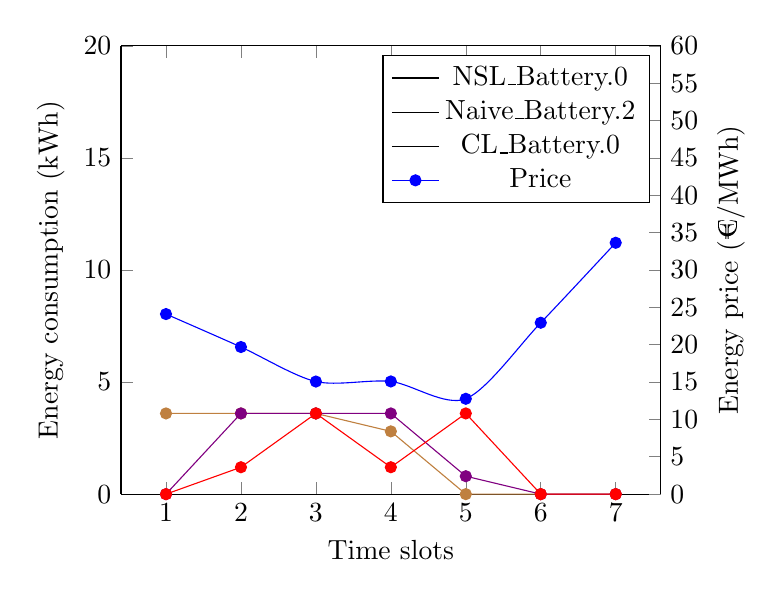
\begin{tikzpicture}
        \begin{axis}[
          axis y line*=left,
          xlabel=Time slots,
          ylabel=Energy consumption (kWh),
          ymin=0, ymax=20
        ]
        
        \addplot[mark=*, brown]
          coordinates{
            (1,3.6)
            (2,3.6)
            (3,3.6)
            (4,2.8)
            (5,0)
            (6,0)
            (7,0)
        }; \label{NSL}
        
        \addplot[mark=*, violet]
          coordinates{
            (1,0)
            (2,3.6)
            (3,3.6)
            (4,3.6)
            (5,0.8)
            (6,0)
            (7,0)
        }; \label{Naive}
        
        \addplot[mark=*,red]
          coordinates{
            (1,0.0)
            (2,1.2)
            (3,3.6)
            (4,1.2)
            (5,3.6)
            (6,0)
            (7,0)
        }; \label{CL}
        
        \end{axis}
        
        \begin{axis}[
          axis y line*=right,
          axis x line=none,
          ymin=0, ymax=60,
          ytick={0,5,10,15,20,25,30,35,40, 45, 50, 55, 60},
          ylabel= Energy price (€/MWh)
        ]
        \addlegendimage{/pgfplots/refstyle=NSL}\addlegendentry{NSL\_Battery.0}
        \addlegendimage{/pgfplots/refstyle=Naive}\addlegendentry{Naive\_Battery.2}
        \addlegendimage{/pgfplots/refstyle=CL}\addlegendentry{CL\_Battery.0}
        
        \addplot[smooth,mark=*,blue]
          coordinates{
            (1,24.10)
            (2,19.69)
            (3,15.07)
            (4,15.08)
            (5,12.76)
            (6,22.94)
            (7,33.64)

        }; \addlegendentry{Price}
        \end{axis}
        \end{tikzpicture}
        \caption{}
    \end{subfigure}
    
    
    
    
    \begin{subfigure}[]{0.7\textwidth}
        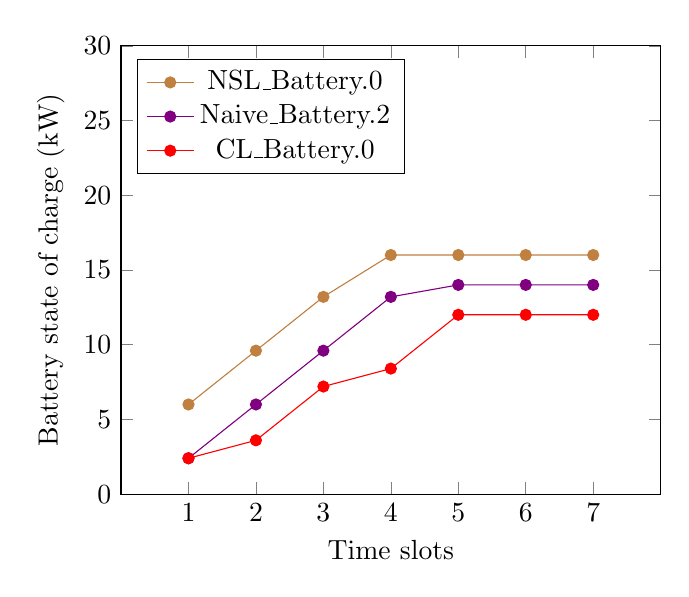
\begin{tikzpicture}
            \begin{axis}[
                xlabel={Time slots},
                ylabel={Battery state of charge (kW)},
                xmin=0, xmax=8,
                ymin=0, ymax=30,
                xtick={1,2,3,4,5,6,7},
                ytick={0,5,10,15,20,25,30},
                legend pos=north west,
            ]
    
                \addplot[
                    color=brown,
                    mark=*,
                    ]
                    coordinates {
                    (1,6.0)(2,9.6)(3,13.2)(4,16)(5,16)(6,16)(7,16)
                    };
                    \addlegendentry{NSL\_Battery.0}
                
                \addplot[
                    color=violet,
                    mark=*,
                    ]
                    coordinates {
                    (1,2.4)(2,6.0)(3,9.6)(4,13.2)(5,14.0)(6,14.0)(7,14.0)
                    };
                    \addlegendentry{Naive\_Battery.2}
                    
                \addplot[
                    color=red,
                    mark=*,
                    ]
                    coordinates {
                    (1,2.4)(2,3.6)(3,7.2)(4,8.4)(5,12.0)(6,12.0)(7,12.0)
                    };
                    \addlegendentry{CL\_Battery.0}
            \end{axis}
        \end{tikzpicture}
        \caption{}
    \end{subfigure}
    

    
\caption{Battery PEV charge with $\rho = 0.2$}
\label{fig:scen1}
\end{figure}

Here are some points to consider:
\begin{itemize}
    \item NSL\_Battery.0 charges the battery at full power as soon as the charge cycle begins, and continues to do so until the battery's state of charge reaches maximum capacity;
    \item Naive\_Battery.2 charges in hours that are less expensive than the battery in terms of price;
    \item Due to the high cost of energy, CL\_Battery.0 does not charge in the first time slot and modulates the demand for energy consumption in the following hours where the price is lower.
\end{itemize}

